\documentclass[1p]{elsarticle_modified}
%\bibliographystyle{elsarticle-num}

%\usepackage[colorlinks]{hyperref}
%\usepackage{abbrmath_seonhwa} %\Abb, \Ascr, \Acal ,\Abf, \Afrak
\usepackage{amsfonts}
\usepackage{amssymb}
\usepackage{amsmath}
\usepackage{amsthm}
\usepackage{scalefnt}
\usepackage{amsbsy}
\usepackage{kotex}
\usepackage{caption}
\usepackage{subfig}
\usepackage{color}
\usepackage{graphicx}
\usepackage{xcolor} %% white, black, red, green, blue, cyan, magenta, yellow
\usepackage{float}
\usepackage{setspace}
\usepackage{hyperref}

\usepackage{tikz}
\usetikzlibrary{arrows}

\usepackage{multirow}
\usepackage{array} % fixed length table
\usepackage{hhline}

%%%%%%%%%%%%%%%%%%%%%
\makeatletter
\renewcommand*\env@matrix[1][\arraystretch]{%
	\edef\arraystretch{#1}%
	\hskip -\arraycolsep
	\let\@ifnextchar\new@ifnextchar
	\array{*\c@MaxMatrixCols c}}
\makeatother %https://tex.stackexchange.com/questions/14071/how-can-i-increase-the-line-spacing-in-a-matrix
%%%%%%%%%%%%%%%

\usepackage[normalem]{ulem}

\newcommand{\msout}[1]{\ifmmode\text{\sout{\ensuremath{#1}}}\else\sout{#1}\fi}
%SOURCE: \msout is \stkout macro in https://tex.stackexchange.com/questions/20609/strikeout-in-math-mode

\newcommand{\cancel}[1]{
	\ifmmode
	{\color{red}\msout{#1}}
	\else
	{\color{red}\sout{#1}}
	\fi
}

\newcommand{\add}[1]{
	{\color{blue}\uwave{#1}}
}

\newcommand{\replace}[2]{
	\ifmmode
	{\color{red}\msout{#1}}{\color{blue}\uwave{#2}}
	\else
	{\color{red}\sout{#1}}{\color{blue}\uwave{#2}}
	\fi
}

\newcommand{\Sol}{\mathcal{S}} %segment
\newcommand{\D}{D} %diagram
\newcommand{\A}{\mathcal{A}} %arc


%%%%%%%%%%%%%%%%%%%%%%%%%%%%%5 test

\def\sl{\operatorname{\textup{SL}}(2,\Cbb)}
\def\psl{\operatorname{\textup{PSL}}(2,\Cbb)}
\def\quan{\mkern 1mu \triangleright \mkern 1mu}

\theoremstyle{definition}
\newtheorem{thm}{Theorem}[section]
\newtheorem{prop}[thm]{Proposition}
\newtheorem{lem}[thm]{Lemma}
\newtheorem{ques}[thm]{Question}
\newtheorem{cor}[thm]{Corollary}
\newtheorem{defn}[thm]{Definition}
\newtheorem{exam}[thm]{Example}
\newtheorem{rmk}[thm]{Remark}
\newtheorem{alg}[thm]{Algorithm}

\newcommand{\I}{\sqrt{-1}}
\begin{document}

%\begin{frontmatter}
%
%\title{Boundary parabolic representations of knots up to 8 crossings}
%
%%% Group authors per affiliation:
%\author{Yunhi Cho} 
%\address{Department of Mathematics, University of Seoul, Seoul, Korea}
%\ead{yhcho@uos.ac.kr}
%
%
%\author{Seonhwa Kim} %\fnref{s_kim}}
%\address{Center for Geometry and Physics, Institute for Basic Science, Pohang, 37673, Korea}
%\ead{ryeona17@ibs.re.kr}
%
%\author{Hyuk Kim}
%\address{Department of Mathematical Sciences, Seoul National University, Seoul 08826, Korea}
%\ead{hyukkim@snu.ac.kr}
%
%\author{Seokbeom Yoon}
%\address{Department of Mathematical Sciences, Seoul National University, Seoul, 08826,  Korea}
%\ead{sbyoon15@snu.ac.kr}
%
%\begin{abstract}
%We find all boundary parabolic representation of knots up to 8 crossings.
%
%\end{abstract}
%\begin{keyword}
%    \MSC[2010] 57M25 
%\end{keyword}
%
%\end{frontmatter}

%\linenumbers
%\tableofcontents
%
\newcommand\colored[1]{\textcolor{white}{\rule[-0.35ex]{0.8em}{1.4ex}}\kern-0.8em\color{red} #1}%
%\newcommand\colored[1]{\textcolor{white}{ #1}\kern-2.17ex	\textcolor{white}{ #1}\kern-1.81ex	\textcolor{white}{ #1}\kern-2.15ex\color{red}#1	}

{\Large $\underline{11n_{94}~(K11n_{94})}$}

\setlength{\tabcolsep}{10pt}
\renewcommand{\arraystretch}{1.6}
\vspace{1cm}\begin{tabular}{m{100pt}>{\centering\arraybackslash}m{274pt}}
\multirow{5}{120pt}{
	\centering
	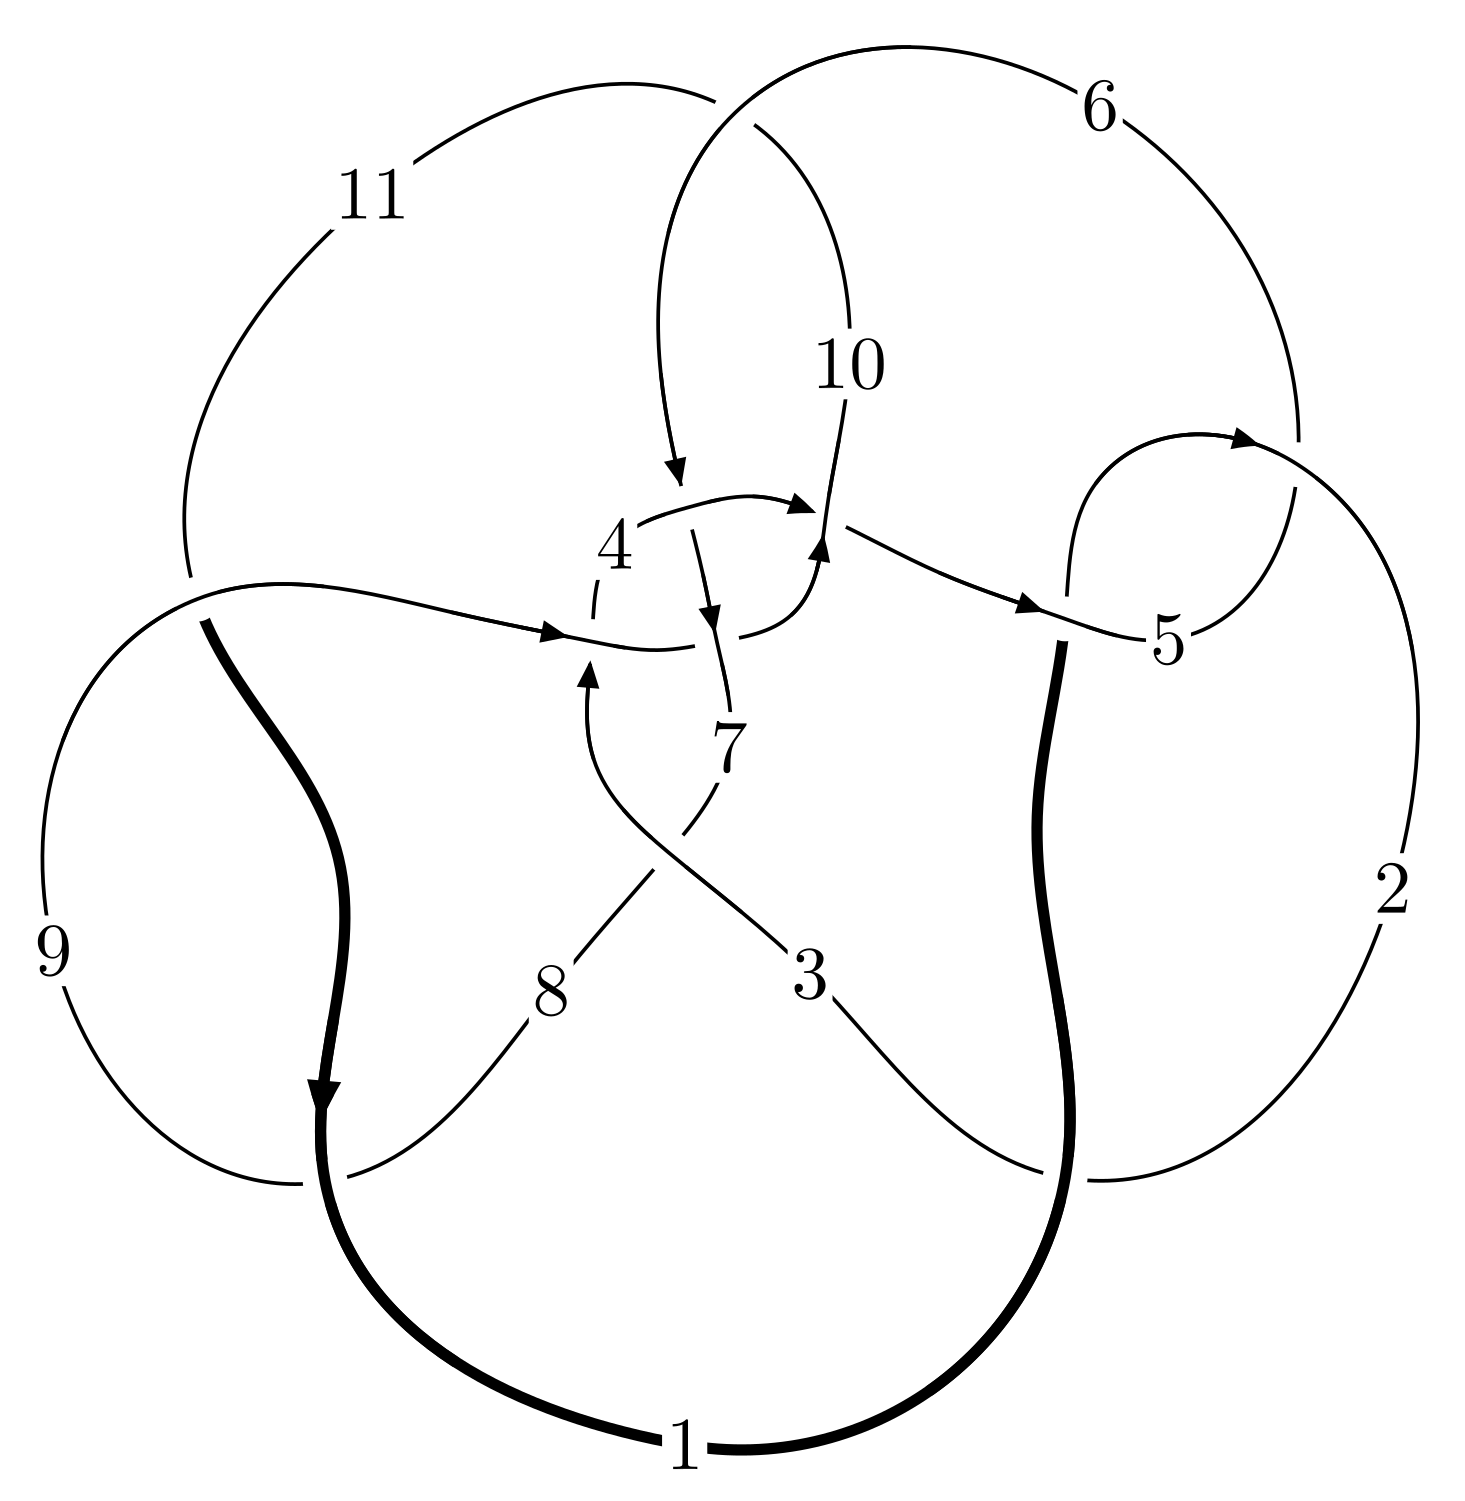
\includegraphics[width=112pt]{../../../GIT/diagram.site/Diagrams/png/710_11n_94.png}\\
\ \ \ A knot diagram\footnotemark}&
\allowdisplaybreaks
\textbf{Linearized knot diagam} \\
\cline{2-2}
 &
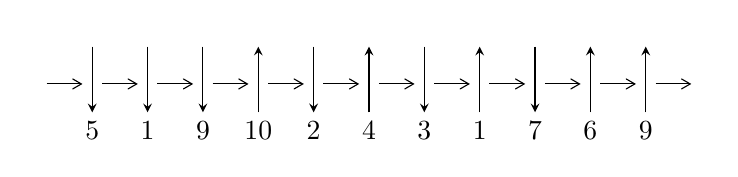
\begin{tikzpicture}[x=20pt, y=17pt]
	% nodes
	\node (C0) at (0, 0) {};
	\node (C1) at (1, 0) {};
	\node (C1U) at (1, +1) {};
	\node (C1D) at (1, -1) {5};

	\node (C2) at (2, 0) {};
	\node (C2U) at (2, +1) {};
	\node (C2D) at (2, -1) {1};

	\node (C3) at (3, 0) {};
	\node (C3U) at (3, +1) {};
	\node (C3D) at (3, -1) {9};

	\node (C4) at (4, 0) {};
	\node (C4U) at (4, +1) {};
	\node (C4D) at (4, -1) {10};

	\node (C5) at (5, 0) {};
	\node (C5U) at (5, +1) {};
	\node (C5D) at (5, -1) {2};

	\node (C6) at (6, 0) {};
	\node (C6U) at (6, +1) {};
	\node (C6D) at (6, -1) {4};

	\node (C7) at (7, 0) {};
	\node (C7U) at (7, +1) {};
	\node (C7D) at (7, -1) {3};

	\node (C8) at (8, 0) {};
	\node (C8U) at (8, +1) {};
	\node (C8D) at (8, -1) {1};

	\node (C9) at (9, 0) {};
	\node (C9U) at (9, +1) {};
	\node (C9D) at (9, -1) {7};

	\node (C10) at (10, 0) {};
	\node (C10U) at (10, +1) {};
	\node (C10D) at (10, -1) {6};

	\node (C11) at (11, 0) {};
	\node (C11U) at (11, +1) {};
	\node (C11D) at (11, -1) {9};
	\node (C12) at (12, 0) {};

	% arrows
	\draw[->,>={angle 60}]
	(C0) edge (C1) (C1) edge (C2) (C2) edge (C3) (C3) edge (C4) (C4) edge (C5) (C5) edge (C6) (C6) edge (C7) (C7) edge (C8) (C8) edge (C9) (C9) edge (C10) (C10) edge (C11) (C11) edge (C12) ;	\draw[->,>=stealth]
	(C1U) edge (C1D) (C2U) edge (C2D) (C3U) edge (C3D) (C4D) edge (C4U) (C5U) edge (C5D) (C6D) edge (C6U) (C7U) edge (C7D) (C8D) edge (C8U) (C9U) edge (C9D) (C10D) edge (C10U) (C11D) edge (C11U) ;
	\end{tikzpicture} \\
\hhline{~~} \\& 
\textbf{Solving Sequence} \\ \cline{2-2} 
 &
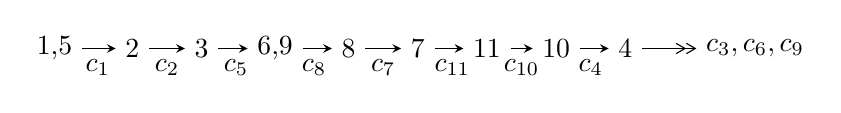
\begin{tikzpicture}[x=25pt, y=7pt]
	% node
	\node (A0) at (-1/8, 0) {1,5};
	\node (A1) at (1, 0) {2};
	\node (A2) at (2, 0) {3};
	\node (A3) at (49/16, 0) {6,9};
	\node (A4) at (33/8, 0) {8};
	\node (A5) at (41/8, 0) {7};
	\node (A6) at (49/8, 0) {11};
	\node (A7) at (57/8, 0) {10};
	\node (A8) at (65/8, 0) {4};
	\node (C1) at (1/2, -1) {$c_{1}$};
	\node (C2) at (3/2, -1) {$c_{2}$};
	\node (C3) at (5/2, -1) {$c_{5}$};
	\node (C4) at (29/8, -1) {$c_{8}$};
	\node (C5) at (37/8, -1) {$c_{7}$};
	\node (C6) at (45/8, -1) {$c_{11}$};
	\node (C7) at (53/8, -1) {$c_{10}$};
	\node (C8) at (61/8, -1) {$c_{4}$};
	\node (A9) at (10, 0) {$c_{3},c_{6},c_{9}$};

	% edge
	\draw[->,>=stealth]	
	(A0) edge (A1) (A1) edge (A2) (A2) edge (A3) (A3) edge (A4) (A4) edge (A5) (A5) edge (A6) (A6) edge (A7) (A7) edge (A8) ;
	\draw[->>,>={angle 60}]	
	(A8) edge (A9);
\end{tikzpicture} \\ 

\end{tabular} \\

\footnotetext{
The image of knot diagram is generated by the software ``\textbf{Draw programme}" developed by Andrew Bartholomew(\url{http://www.layer8.co.uk/maths/draw/index.htm\#Running-draw}), where we modified some parts for our purpose(\url{https://github.com/CATsTAILs/LinksPainter}).
}\phantom \\ \newline 
\centering \textbf{Ideals for irreducible components\footnotemark of $X_{\text{par}}$} 
 
\begin{align*}
I^u_{1}&=\langle 
16 u^{18}-65 u^{17}+\cdots+39 b+33,\;-20 u^{18}+91 u^{17}+\cdots+39 a-129,\;u^{19}-5 u^{18}+\cdots+10 u^2-3\rangle \\
I^u_{2}&=\langle 
u^9+2 u^8-4 u^6-2 u^5+4 u^4+3 u^3- u^2+b+1,\;- u^9-2 u^8+u^7+5 u^6+u^5-7 u^4-3 u^3+4 u^2+a+u-2,\\
\phantom{I^u_{2}}&\phantom{= \langle  }u^{10}+2 u^9-4 u^7-2 u^6+4 u^5+4 u^4- u^3- u^2+u+1\rangle \\
I^u_{3}&=\langle 
-2 u^9-3 u^8- u^7+5 u^6-3 u^4- u^2 a-2 u^3- a u+6 u^2+b-2 u-3,\;-3 u^9 a+2 u^9+\cdots-4 a+2,\\
\phantom{I^u_{3}}&\phantom{= \langle  }u^{10}+2 u^9+u^8-3 u^7-2 u^6+2 u^5+3 u^4-2 u^3- u^2+2 u+1\rangle \\
I^u_{4}&=\langle 
b-1,\;a^2- a-1,\;u-1\rangle \\
\\
I^v_{1}&=\langle 
a,\;b-1,\;v-1\rangle \\
\end{align*}
\raggedright * 5 irreducible components of $\dim_{\mathbb{C}}=0$, with total 52 representations.\\
\footnotetext{All coefficients of polynomials are rational numbers. But the coefficients are sometimes approximated in decimal forms when there is not enough margin.}
\newpage
\renewcommand{\arraystretch}{1}
\centering \section*{I. $I^u_{1}= \langle 16 u^{18}-65 u^{17}+\cdots+39 b+33,\;-20 u^{18}+91 u^{17}+\cdots+39 a-129,\;u^{19}-5 u^{18}+\cdots+10 u^2-3 \rangle$}
\flushleft \textbf{(i) Arc colorings}\\
\begin{tabular}{m{7pt} m{180pt} m{7pt} m{180pt} }
\flushright $a_{1}=$&$\begin{pmatrix}1\\0\end{pmatrix}$ \\
\flushright $a_{5}=$&$\begin{pmatrix}0\\u\end{pmatrix}$ \\
\flushright $a_{2}=$&$\begin{pmatrix}1\\u^2\end{pmatrix}$ \\
\flushright $a_{3}=$&$\begin{pmatrix}- u^2+1\\u^2\end{pmatrix}$ \\
\flushright $a_{6}=$&$\begin{pmatrix}- u\\- u^3+u\end{pmatrix}$ \\
\flushright $a_{9}=$&$\begin{pmatrix}0.512821 u^{18}-2.33333 u^{17}+\cdots+2.12821 u+3.30769\\-0.410256 u^{18}+1.66667 u^{17}+\cdots-1.76923 u-0.846154\end{pmatrix}$ \\
\flushright $a_{8}=$&$\begin{pmatrix}0.923077 u^{18}-4 u^{17}+\cdots+3.89744 u+4.15385\\-0.410256 u^{18}+1.66667 u^{17}+\cdots-1.76923 u-0.846154\end{pmatrix}$ \\
\flushright $a_{7}=$&$\begin{pmatrix}\frac{5}{39} u^{18}- u^{17}+\cdots+\frac{50}{39} u+\frac{27}{13}\\0.153846 u^{18}-0.794872 u^{16}+\cdots-2.46154 u-0.307692\end{pmatrix}$ \\
\flushright $a_{11}=$&$\begin{pmatrix}1.10256 u^{18}-8 u^{17}+\cdots+7.35897 u+10.4615\\-3.94872 u^{18}+18.3333 u^{17}+\cdots-6.15385 u-10.7692\end{pmatrix}$ \\
\flushright $a_{10}=$&$\begin{pmatrix}-0.307692 u^{18}+2.66667 u^{17}+\cdots-3.41026 u-1.38462\\6.20513 u^{18}-25.6667 u^{17}+\cdots+0.384615 u+11.9231\end{pmatrix}$ \\
\flushright $a_{4}=$&$\begin{pmatrix}1.41026 u^{18}-5.33333 u^{17}+\cdots-1.56410 u+2.84615\\-1.12821 u^{18}+3.33333 u^{17}+\cdots+2.38462 u+0.923077\end{pmatrix}$\\ \flushright $a_{4}=$&$\begin{pmatrix}1.41026 u^{18}-5.33333 u^{17}+\cdots-1.56410 u+2.84615\\-1.12821 u^{18}+3.33333 u^{17}+\cdots+2.38462 u+0.923077\end{pmatrix}$\\&\end{tabular}
\flushleft \textbf{(ii) Obstruction class $= -1$}\\~\\
\flushleft \textbf{(iii) Cusp Shapes $= \frac{389}{39} u^{18}-\frac{140}{3} u^{17}+\cdots-\frac{38}{13} u+\frac{356}{13}$}\\~\\
\newpage\renewcommand{\arraystretch}{1}
\flushleft \textbf{(iv) u-Polynomials at the component}\newline \\
\begin{tabular}{m{50pt}|m{274pt}}
Crossings & \hspace{64pt}u-Polynomials at each crossing \\
\hline $$\begin{aligned}c_{1},c_{5}\end{aligned}$$&$\begin{aligned}
&u^{19}+5 u^{18}+\cdots-10 u^2+3
\end{aligned}$\\
\hline $$\begin{aligned}c_{2}\end{aligned}$$&$\begin{aligned}
&u^{19}+5 u^{18}+\cdots+60 u+9
\end{aligned}$\\
\hline $$\begin{aligned}c_{3}\end{aligned}$$&$\begin{aligned}
&u^{19}+8 u^{17}+\cdots- u+5
\end{aligned}$\\
\hline $$\begin{aligned}c_{4},c_{6}\end{aligned}$$&$\begin{aligned}
&u^{19}+u^{18}+\cdots+4 u+1
\end{aligned}$\\
\hline $$\begin{aligned}c_{7}\end{aligned}$$&$\begin{aligned}
&u^{19}+20 u^{17}+\cdots+3 u+1
\end{aligned}$\\
\hline $$\begin{aligned}c_{8},c_{11}\end{aligned}$$&$\begin{aligned}
&u^{19}-18 u^{17}+\cdots+13 u+1
\end{aligned}$\\
\hline $$\begin{aligned}c_{9}\end{aligned}$$&$\begin{aligned}
&u^{19}-14 u^{18}+\cdots-30 u+3
\end{aligned}$\\
\hline $$\begin{aligned}c_{10}\end{aligned}$$&$\begin{aligned}
&u^{19}-21 u^{18}+\cdots-1792 u+512
\end{aligned}$\\
\hline
\end{tabular}\\~\\
\newpage\renewcommand{\arraystretch}{1}
\flushleft \textbf{(v) Riley Polynomials at the component}\newline \\
\begin{tabular}{m{50pt}|m{274pt}}
Crossings & \hspace{64pt}Riley Polynomials at each crossing \\
\hline $$\begin{aligned}c_{1},c_{5}\end{aligned}$$&$\begin{aligned}
&y^{19}-5 y^{18}+\cdots+60 y-9
\end{aligned}$\\
\hline $$\begin{aligned}c_{2}\end{aligned}$$&$\begin{aligned}
&y^{19}+23 y^{18}+\cdots-1872 y-81
\end{aligned}$\\
\hline $$\begin{aligned}c_{3}\end{aligned}$$&$\begin{aligned}
&y^{19}+16 y^{18}+\cdots-109 y-25
\end{aligned}$\\
\hline $$\begin{aligned}c_{4},c_{6}\end{aligned}$$&$\begin{aligned}
&y^{19}-7 y^{18}+\cdots+16 y-1
\end{aligned}$\\
\hline $$\begin{aligned}c_{7}\end{aligned}$$&$\begin{aligned}
&y^{19}+40 y^{18}+\cdots+7 y-1
\end{aligned}$\\
\hline $$\begin{aligned}c_{8},c_{11}\end{aligned}$$&$\begin{aligned}
&y^{19}-36 y^{18}+\cdots+39 y-1
\end{aligned}$\\
\hline $$\begin{aligned}c_{9}\end{aligned}$$&$\begin{aligned}
&y^{19}+38 y^{17}+\cdots+42 y-9
\end{aligned}$\\
\hline $$\begin{aligned}c_{10}\end{aligned}$$&$\begin{aligned}
&y^{19}-9 y^{18}+\cdots+2162688 y-262144
\end{aligned}$\\
\hline
\end{tabular}\\~\\
\newpage\flushleft \textbf{(vi) Complex Volumes and Cusp Shapes}
$$\begin{array}{c|c|c}  
\text{Solutions to }I^u_{1}& \I (\text{vol} + \sqrt{-1}CS) & \text{Cusp shape}\\
 \hline 
\begin{aligned}
u &= -0.350966 + 0.908273 I \\
a &= \phantom{-}0.497187 - 0.151368 I \\
b &= -0.408408 - 0.715459 I\end{aligned}
 & \phantom{-}2.38098 - 2.19136 I & \phantom{-}4.02486 + 1.79521 I \\ \hline\begin{aligned}
u &= -0.350966 - 0.908273 I \\
a &= \phantom{-}0.497187 + 0.151368 I \\
b &= -0.408408 + 0.715459 I\end{aligned}
 & \phantom{-}2.38098 + 2.19136 I & \phantom{-}4.02486 - 1.79521 I \\ \hline\begin{aligned}
u &= -0.779496 + 0.468978 I \\
a &= -0.091107 + 0.590275 I \\
b &= \phantom{-}0.602057 + 0.798290 I\end{aligned}
 & \phantom{-}0.99904 + 3.33102 I & \phantom{-}2.55789 - 7.26755 I \\ \hline\begin{aligned}
u &= -0.779496 - 0.468978 I \\
a &= -0.091107 - 0.590275 I \\
b &= \phantom{-}0.602057 - 0.798290 I\end{aligned}
 & \phantom{-}0.99904 - 3.33102 I & \phantom{-}2.55789 + 7.26755 I \\ \hline\begin{aligned}
u &= \phantom{-}1.077080 + 0.271096 I \\
a &= \phantom{-}0.401351 + 0.468581 I \\
b &= -0.142788 + 0.130045 I\end{aligned}
 & -2.28578 - 0.47591 I & -3.82840 + 3.46313 I \\ \hline\begin{aligned}
u &= \phantom{-}1.077080 - 0.271096 I \\
a &= \phantom{-}0.401351 - 0.468581 I \\
b &= -0.142788 - 0.130045 I\end{aligned}
 & -2.28578 + 0.47591 I & -3.82840 - 3.46313 I \\ \hline\begin{aligned}
u &= \phantom{-}0.761451\phantom{ +0.000000I} \\
a &= \phantom{-}1.02355\phantom{ +0.000000I} \\
b &= -0.185922\phantom{ +0.000000I}\end{aligned}
 & -1.28421\phantom{ +0.000000I} & -7.36270\phantom{ +0.000000I} \\ \hline\begin{aligned}
u &= \phantom{-}0.898363 + 0.894383 I \\
a &= -1.77752 - 0.80237 I \\
b &= \phantom{-}2.15592 - 0.55152 I\end{aligned}
 & \phantom{-}8.84727 - 4.55297 I & \phantom{-}5.83723 + 8.19473 I \\ \hline\begin{aligned}
u &= \phantom{-}0.898363 - 0.894383 I \\
a &= -1.77752 + 0.80237 I \\
b &= \phantom{-}2.15592 + 0.55152 I\end{aligned}
 & \phantom{-}8.84727 + 4.55297 I & \phantom{-}5.83723 - 8.19473 I \\ \hline\begin{aligned}
u &= \phantom{-}0.956723 + 0.863236 I \\
a &= -1.21407 - 1.44574 I \\
b &= \phantom{-}2.09496 + 0.17987 I\end{aligned}
 & \phantom{-}8.65502 - 1.95883 I & \phantom{-}4.78017 - 2.64502 I\\
 \hline 
 \end{array}$$\newpage$$\begin{array}{c|c|c}  
\text{Solutions to }I^u_{1}& \I (\text{vol} + \sqrt{-1}CS) & \text{Cusp shape}\\
 \hline 
\begin{aligned}
u &= \phantom{-}0.956723 - 0.863236 I \\
a &= -1.21407 + 1.44574 I \\
b &= \phantom{-}2.09496 - 0.17987 I\end{aligned}
 & \phantom{-}8.65502 + 1.95883 I & \phantom{-}4.78017 + 2.64502 I \\ \hline\begin{aligned}
u &= -1.200480 + 0.502359 I \\
a &= -0.256728 - 0.089743 I \\
b &= -0.766723 + 0.224201 I\end{aligned}
 & -0.51529 + 7.49251 I & \phantom{-}1.46560 - 6.64058 I \\ \hline\begin{aligned}
u &= -1.200480 - 0.502359 I \\
a &= -0.256728 + 0.089743 I \\
b &= -0.766723 - 0.224201 I\end{aligned}
 & -0.51529 - 7.49251 I & \phantom{-}1.46560 + 6.64058 I \\ \hline\begin{aligned}
u &= \phantom{-}0.869568 + 1.036960 I \\
a &= \phantom{-}1.19820 + 0.93760 I \\
b &= -2.14294 - 0.19617 I\end{aligned}
 & \phantom{-}10.89150 + 6.89079 I & \phantom{-}1.93588 - 3.17270 I \\ \hline\begin{aligned}
u &= \phantom{-}0.869568 - 1.036960 I \\
a &= \phantom{-}1.19820 - 0.93760 I \\
b &= -2.14294 + 0.19617 I\end{aligned}
 & \phantom{-}10.89150 - 6.89079 I & \phantom{-}1.93588 + 3.17270 I \\ \hline\begin{aligned}
u &= \phantom{-}1.063600 + 0.913849 I \\
a &= \phantom{-}1.35608 + 1.04713 I \\
b &= -2.11940 + 0.59325 I\end{aligned}
 & \phantom{-}10.2390 - 14.0065 I & \phantom{-}0.95958 + 7.34096 I \\ \hline\begin{aligned}
u &= \phantom{-}1.063600 - 0.913849 I \\
a &= \phantom{-}1.35608 - 1.04713 I \\
b &= -2.11940 - 0.59325 I\end{aligned}
 & \phantom{-}10.2390 + 14.0065 I & \phantom{-}0.95958 - 7.34096 I \\ \hline\begin{aligned}
u &= -0.415119 + 0.278912 I \\
a &= \phantom{-}0.874831 + 0.733477 I \\
b &= \phantom{-}0.820280 - 0.072764 I\end{aligned}
 & \phantom{-}1.73128 - 0.06651 I & \phantom{-}5.44854 - 0.44003 I \\ \hline\begin{aligned}
u &= -0.415119 - 0.278912 I \\
a &= \phantom{-}0.874831 - 0.733477 I \\
b &= \phantom{-}0.820280 + 0.072764 I\end{aligned}
 & \phantom{-}1.73128 + 0.06651 I & \phantom{-}5.44854 + 0.44003 I\\
 \hline 
 \end{array}$$\newpage\newpage\renewcommand{\arraystretch}{1}
\centering \section*{II. $I^u_{2}= \langle u^9+2 u^8-4 u^6-2 u^5+4 u^4+3 u^3- u^2+b+1,\;- u^9-2 u^8+\cdots+a-2,\;u^{10}+2 u^9+\cdots+u+1 \rangle$}
\flushleft \textbf{(i) Arc colorings}\\
\begin{tabular}{m{7pt} m{180pt} m{7pt} m{180pt} }
\flushright $a_{1}=$&$\begin{pmatrix}1\\0\end{pmatrix}$ \\
\flushright $a_{5}=$&$\begin{pmatrix}0\\u\end{pmatrix}$ \\
\flushright $a_{2}=$&$\begin{pmatrix}1\\u^2\end{pmatrix}$ \\
\flushright $a_{3}=$&$\begin{pmatrix}- u^2+1\\u^2\end{pmatrix}$ \\
\flushright $a_{6}=$&$\begin{pmatrix}- u\\- u^3+u\end{pmatrix}$ \\
\flushright $a_{9}=$&$\begin{pmatrix}u^9+2 u^8- u^7-5 u^6- u^5+7 u^4+3 u^3-4 u^2- u+2\\- u^9-2 u^8+4 u^6+2 u^5-4 u^4-3 u^3+u^2-1\end{pmatrix}$ \\
\flushright $a_{8}=$&$\begin{pmatrix}2 u^9+4 u^8- u^7-9 u^6-3 u^5+11 u^4+6 u^3-5 u^2- u+3\\- u^9-2 u^8+4 u^6+2 u^5-4 u^4-3 u^3+u^2-1\end{pmatrix}$ \\
\flushright $a_{7}=$&$\begin{pmatrix}u^9+2 u^8- u^7-5 u^6- u^5+6 u^4+3 u^3-3 u^2- u+1\\- u^8- u^7+u^6+3 u^5-3 u^3- u^2+u\end{pmatrix}$ \\
\flushright $a_{11}=$&$\begin{pmatrix}- u^9- u^8+2 u^7+3 u^6-3 u^5-4 u^4+2 u^3+3 u^2-2 u\\u^9+u^8-2 u^7-3 u^6+2 u^5+4 u^4-2 u^2\end{pmatrix}$ \\
\flushright $a_{10}=$&$\begin{pmatrix}u^8+u^7- u^6-3 u^5+u^4+3 u^3+u^2- u+1\\- u^9- u^8+u^7+2 u^6- u^5-2 u^4+u^3-2 u-1\end{pmatrix}$ \\
\flushright $a_{4}=$&$\begin{pmatrix}-2 u^9-2 u^8+3 u^7+6 u^6-3 u^5-8 u^4+4 u^2- u-1\\u^9+u^8- u^7-3 u^6+3 u^4+2 u^3\end{pmatrix}$\\ \flushright $a_{4}=$&$\begin{pmatrix}-2 u^9-2 u^8+3 u^7+6 u^6-3 u^5-8 u^4+4 u^2- u-1\\u^9+u^8- u^7-3 u^6+3 u^4+2 u^3\end{pmatrix}$\\&\end{tabular}
\flushleft \textbf{(ii) Obstruction class $= 1$}\\~\\
\flushleft \textbf{(iii) Cusp Shapes $= 6 u^9+13 u^8- u^7-23 u^6-11 u^5+23 u^4+15 u^3-3 u^2+u+5$}\\~\\
\newpage\renewcommand{\arraystretch}{1}
\flushleft \textbf{(iv) u-Polynomials at the component}\newline \\
\begin{tabular}{m{50pt}|m{274pt}}
Crossings & \hspace{64pt}u-Polynomials at each crossing \\
\hline $$\begin{aligned}c_{1}\end{aligned}$$&$\begin{aligned}
&u^{10}+2 u^9-4 u^7-2 u^6+4 u^5+4 u^4- u^3- u^2+u+1
\end{aligned}$\\
\hline $$\begin{aligned}c_{2}\end{aligned}$$&$\begin{aligned}
&u^{10}+4 u^9+\cdots+3 u+1
\end{aligned}$\\
\hline $$\begin{aligned}c_{3}\end{aligned}$$&$\begin{aligned}
&u^{10}+u^9+3 u^8+2 u^7+3 u^6+u^5+3 u^4+u^3+u^2+1
\end{aligned}$\\
\hline $$\begin{aligned}c_{4},c_{6}\end{aligned}$$&$\begin{aligned}
&u^{10}+u^8- u^7+3 u^6- u^5+3 u^4-2 u^3+3 u^2- u+1
\end{aligned}$\\
\hline $$\begin{aligned}c_{5}\end{aligned}$$&$\begin{aligned}
&u^{10}-2 u^9+4 u^7-2 u^6-4 u^5+4 u^4+u^3- u^2- u+1
\end{aligned}$\\
\hline $$\begin{aligned}c_{7}\end{aligned}$$&$\begin{aligned}
&u^{10}+u^9+3 u^8-8 u^6+3 u^5+9 u^4+6 u^3+9 u^2+4 u+1
\end{aligned}$\\
\hline $$\begin{aligned}c_{8}\end{aligned}$$&$\begin{aligned}
&u^{10}+5 u^9+11 u^8+18 u^7+23 u^6+21 u^5+19 u^4+11 u^3+7 u^2+2 u+1
\end{aligned}$\\
\hline $$\begin{aligned}c_{9}\end{aligned}$$&$\begin{aligned}
&u^{10}+5 u^9+11 u^8+10 u^7-5 u^6-23 u^5-21 u^4+u^3+18 u^2+15 u+5
\end{aligned}$\\
\hline $$\begin{aligned}c_{10}\end{aligned}$$&$\begin{aligned}
&u^{10}+3 u^9-11 u^7-14 u^6+4 u^5+20 u^4+14 u^3+5 u^2+2 u+1
\end{aligned}$\\
\hline $$\begin{aligned}c_{11}\end{aligned}$$&$\begin{aligned}
&u^{10}-5 u^9+11 u^8-18 u^7+23 u^6-21 u^5+19 u^4-11 u^3+7 u^2-2 u+1
\end{aligned}$\\
\hline
\end{tabular}\\~\\
\newpage\renewcommand{\arraystretch}{1}
\flushleft \textbf{(v) Riley Polynomials at the component}\newline \\
\begin{tabular}{m{50pt}|m{274pt}}
Crossings & \hspace{64pt}Riley Polynomials at each crossing \\
\hline $$\begin{aligned}c_{1},c_{5}\end{aligned}$$&$\begin{aligned}
&y^{10}-4 y^9+\cdots-3 y+1
\end{aligned}$\\
\hline $$\begin{aligned}c_{2}\end{aligned}$$&$\begin{aligned}
&y^{10}+8 y^9+\cdots+13 y+1
\end{aligned}$\\
\hline $$\begin{aligned}c_{3}\end{aligned}$$&$\begin{aligned}
&y^{10}+5 y^9+11 y^8+18 y^7+23 y^6+21 y^5+19 y^4+11 y^3+7 y^2+2 y+1
\end{aligned}$\\
\hline $$\begin{aligned}c_{4},c_{6}\end{aligned}$$&$\begin{aligned}
&y^{10}+2 y^9+7 y^8+11 y^7+19 y^6+21 y^5+23 y^4+18 y^3+11 y^2+5 y+1
\end{aligned}$\\
\hline $$\begin{aligned}c_{7}\end{aligned}$$&$\begin{aligned}
&y^{10}+5 y^9+\cdots+2 y+1
\end{aligned}$\\
\hline $$\begin{aligned}c_{8},c_{11}\end{aligned}$$&$\begin{aligned}
&y^{10}-3 y^9+\cdots+10 y+1
\end{aligned}$\\
\hline $$\begin{aligned}c_{9}\end{aligned}$$&$\begin{aligned}
&y^{10}-3 y^9+\cdots-45 y+25
\end{aligned}$\\
\hline $$\begin{aligned}c_{10}\end{aligned}$$&$\begin{aligned}
&y^{10}-9 y^9+\cdots+6 y+1
\end{aligned}$\\
\hline
\end{tabular}\\~\\
\newpage\flushleft \textbf{(vi) Complex Volumes and Cusp Shapes}
$$\begin{array}{c|c|c}  
\text{Solutions to }I^u_{2}& \I (\text{vol} + \sqrt{-1}CS) & \text{Cusp shape}\\
 \hline 
\begin{aligned}
u &= -1.032960 + 0.512793 I \\
a &= -0.926519 - 0.444783 I \\
b &= -0.031024 + 0.608247 I\end{aligned}
 & -1.82490 + 7.04514 I & -4.29839 - 6.63243 I \\ \hline\begin{aligned}
u &= -1.032960 - 0.512793 I \\
a &= -0.926519 + 0.444783 I \\
b &= -0.031024 - 0.608247 I\end{aligned}
 & -1.82490 - 7.04514 I & -4.29839 + 6.63243 I \\ \hline\begin{aligned}
u &= \phantom{-}1.081750 + 0.414901 I \\
a &= \phantom{-}0.291782 + 0.133729 I \\
b &= \phantom{-}0.431318 + 0.661100 I\end{aligned}
 & -2.42349 + 0.47280 I & -4.60679 - 3.67832 I \\ \hline\begin{aligned}
u &= \phantom{-}1.081750 - 0.414901 I \\
a &= \phantom{-}0.291782 - 0.133729 I \\
b &= \phantom{-}0.431318 - 0.661100 I\end{aligned}
 & -2.42349 - 0.47280 I & -4.60679 + 3.67832 I \\ \hline\begin{aligned}
u &= -0.620721 + 0.483253 I \\
a &= \phantom{-}0.78365 + 1.55026 I \\
b &= -0.186622 - 0.818442 I\end{aligned}
 & -0.43993 - 2.89386 I & -0.09413 + 2.87221 I \\ \hline\begin{aligned}
u &= -0.620721 - 0.483253 I \\
a &= \phantom{-}0.78365 - 1.55026 I \\
b &= -0.186622 + 0.818442 I\end{aligned}
 & -0.43993 + 2.89386 I & -0.09413 - 2.87221 I \\ \hline\begin{aligned}
u &= \phantom{-}0.517593 + 0.494789 I \\
a &= -0.808469 - 0.682785 I \\
b &= \phantom{-}0.250433 - 1.183290 I\end{aligned}
 & -0.42431 - 4.26902 I & -1.08356 + 8.09272 I \\ \hline\begin{aligned}
u &= \phantom{-}0.517593 - 0.494789 I \\
a &= -0.808469 + 0.682785 I \\
b &= \phantom{-}0.250433 + 1.183290 I\end{aligned}
 & -0.42431 + 4.26902 I & -1.08356 - 8.09272 I \\ \hline\begin{aligned}
u &= -0.945660 + 0.933377 I \\
a &= -1.34045 + 0.96068 I \\
b &= \phantom{-}2.03589 + 0.22886 I\end{aligned}
 & \phantom{-}8.40249 + 3.42159 I & \phantom{-}1.58287 - 2.15087 I \\ \hline\begin{aligned}
u &= -0.945660 - 0.933377 I \\
a &= -1.34045 - 0.96068 I \\
b &= \phantom{-}2.03589 - 0.22886 I\end{aligned}
 & \phantom{-}8.40249 - 3.42159 I & \phantom{-}1.58287 + 2.15087 I\\
 \hline 
 \end{array}$$\newpage\newpage\renewcommand{\arraystretch}{1}
\centering \section*{III. $I^u_{3}= \langle -2 u^9-3 u^8+\cdots+b-3,\;-3 u^9 a+2 u^9+\cdots-4 a+2,\;u^{10}+2 u^9+\cdots+2 u+1 \rangle$}
\flushleft \textbf{(i) Arc colorings}\\
\begin{tabular}{m{7pt} m{180pt} m{7pt} m{180pt} }
\flushright $a_{1}=$&$\begin{pmatrix}1\\0\end{pmatrix}$ \\
\flushright $a_{5}=$&$\begin{pmatrix}0\\u\end{pmatrix}$ \\
\flushright $a_{2}=$&$\begin{pmatrix}1\\u^2\end{pmatrix}$ \\
\flushright $a_{3}=$&$\begin{pmatrix}- u^2+1\\u^2\end{pmatrix}$ \\
\flushright $a_{6}=$&$\begin{pmatrix}- u\\- u^3+u\end{pmatrix}$ \\
\flushright $a_{9}=$&$\begin{pmatrix}a\\2 u^9+3 u^8+u^7-5 u^6+3 u^4+u^2 a+2 u^3+a u-6 u^2+2 u+3\end{pmatrix}$ \\
\flushright $a_{8}=$&$\begin{pmatrix}-2 u^9-3 u^8- u^7+5 u^6-3 u^4- u^2 a-2 u^3- a u+6 u^2+a-2 u-3\\2 u^9+3 u^8+u^7-5 u^6+3 u^4+u^2 a+2 u^3+a u-6 u^2+2 u+3\end{pmatrix}$ \\
\flushright $a_{7}=$&$\begin{pmatrix}- u^9-2 u^8- u^7+3 u^6+2 u^5- u^3 a- u^4- u^2 a-2 u^3+2 u^2+a-1\\3 u^9+5 u^8+\cdots+2 u+4\end{pmatrix}$ \\
\flushright $a_{11}=$&$\begin{pmatrix}u^9 a+u^9+\cdots+2 a+1\\- u^9 a-2 u^9+\cdots- a-3\end{pmatrix}$ \\
\flushright $a_{10}=$&$\begin{pmatrix}u^9 a+u^9+\cdots+2 a+1\\- u^9 a-2 u^9+\cdots- a-3\end{pmatrix}$ \\
\flushright $a_{4}=$&$\begin{pmatrix}2 u^9+3 u^8+\cdots- a+3\\- u^9 a-2 u^9+\cdots- a-3\end{pmatrix}$\\ \flushright $a_{4}=$&$\begin{pmatrix}2 u^9+3 u^8+\cdots- a+3\\- u^9 a-2 u^9+\cdots- a-3\end{pmatrix}$\\&\end{tabular}
\flushleft \textbf{(ii) Obstruction class $= -1$}\\~\\
\flushleft \textbf{(iii) Cusp Shapes $= -11 u^9-17 u^8+37 u^6+3 u^5-35 u^4-20 u^3+38 u^2-3 u-23$}\\~\\
\newpage\renewcommand{\arraystretch}{1}
\flushleft \textbf{(iv) u-Polynomials at the component}\newline \\
\begin{tabular}{m{50pt}|m{274pt}}
Crossings & \hspace{64pt}u-Polynomials at each crossing \\
\hline $$\begin{aligned}c_{1},c_{5}\end{aligned}$$&$\begin{aligned}
&(u^{10}-2 u^9+u^8+3 u^7-2 u^6-2 u^5+3 u^4+2 u^3- u^2-2 u+1)^2
\end{aligned}$\\
\hline $$\begin{aligned}c_{2}\end{aligned}$$&$\begin{aligned}
&(u^{10}+2 u^9+9 u^8+15 u^7+28 u^6+36 u^5+35 u^4+22 u^3+15 u^2+6 u+1)^{2}
\end{aligned}$\\
\hline $$\begin{aligned}c_{3}\end{aligned}$$&$\begin{aligned}
&u^{20}+2 u^{19}+\cdots-301 u+457
\end{aligned}$\\
\hline $$\begin{aligned}c_{4},c_{6}\end{aligned}$$&$\begin{aligned}
&u^{20}+2 u^{19}+\cdots-5 u+5
\end{aligned}$\\
\hline $$\begin{aligned}c_{7}\end{aligned}$$&$\begin{aligned}
&u^{20}+12 u^{18}+\cdots-989 u+1201
\end{aligned}$\\
\hline $$\begin{aligned}c_{8},c_{11}\end{aligned}$$&$\begin{aligned}
&u^{20}-3 u^{19}+\cdots+410 u+55
\end{aligned}$\\
\hline $$\begin{aligned}c_{9}\end{aligned}$$&$\begin{aligned}
&(u^{10}+3 u^9+6 u^8+7 u^7+9 u^6+9 u^5+10 u^4+6 u^3+5 u^2+3 u+2)^2
\end{aligned}$\\
\hline $$\begin{aligned}c_{10}\end{aligned}$$&$\begin{aligned}
&(u+1)^{20}
\end{aligned}$\\
\hline
\end{tabular}\\~\\
\newpage\renewcommand{\arraystretch}{1}
\flushleft \textbf{(v) Riley Polynomials at the component}\newline \\
\begin{tabular}{m{50pt}|m{274pt}}
Crossings & \hspace{64pt}Riley Polynomials at each crossing \\
\hline $$\begin{aligned}c_{1},c_{5}\end{aligned}$$&$\begin{aligned}
&(y^{10}-2 y^9+9 y^8-15 y^7+28 y^6-36 y^5+35 y^4-22 y^3+15 y^2-6 y+1)^{2}
\end{aligned}$\\
\hline $$\begin{aligned}c_{2}\end{aligned}$$&$\begin{aligned}
&(y^{10}+14 y^9+\cdots-6 y+1)^{2}
\end{aligned}$\\
\hline $$\begin{aligned}c_{3}\end{aligned}$$&$\begin{aligned}
&y^{20}+12 y^{19}+\cdots-305391 y+208849
\end{aligned}$\\
\hline $$\begin{aligned}c_{4},c_{6}\end{aligned}$$&$\begin{aligned}
&y^{20}+28 y^{18}+\cdots-275 y+25
\end{aligned}$\\
\hline $$\begin{aligned}c_{7}\end{aligned}$$&$\begin{aligned}
&y^{20}+24 y^{19}+\cdots-10199399 y+1442401
\end{aligned}$\\
\hline $$\begin{aligned}c_{8},c_{11}\end{aligned}$$&$\begin{aligned}
&y^{20}-23 y^{19}+\cdots-8050 y+3025
\end{aligned}$\\
\hline $$\begin{aligned}c_{9}\end{aligned}$$&$\begin{aligned}
&(y^{10}+3 y^9+\cdots+11 y+4)^{2}
\end{aligned}$\\
\hline $$\begin{aligned}c_{10}\end{aligned}$$&$\begin{aligned}
&(y-1)^{20}
\end{aligned}$\\
\hline
\end{tabular}\\~\\
\newpage\flushleft \textbf{(vi) Complex Volumes and Cusp Shapes}
$$\begin{array}{c|c|c}  
\text{Solutions to }I^u_{3}& \I (\text{vol} + \sqrt{-1}CS) & \text{Cusp shape}\\
 \hline 
\begin{aligned}
u &= \phantom{-}0.975430 + 0.320615 I \\
a &= \phantom{-}0.583170 - 0.332488 I \\
b &= -0.819443 + 0.010673 I\end{aligned}
 & -0.581891 + 0.600845 I & -1.31849 - 3.40041 I \\ \hline\begin{aligned}
u &= \phantom{-}0.975430 + 0.320615 I \\
a &= \phantom{-}1.43037 - 0.39642 I \\
b &= \phantom{-}0.786422 + 0.695571 I\end{aligned}
 & -0.581891 + 0.600845 I & -1.31849 - 3.40041 I \\ \hline\begin{aligned}
u &= \phantom{-}0.975430 - 0.320615 I \\
a &= \phantom{-}0.583170 + 0.332488 I \\
b &= -0.819443 - 0.010673 I\end{aligned}
 & -0.581891 - 0.600845 I & -1.31849 + 3.40041 I \\ \hline\begin{aligned}
u &= \phantom{-}0.975430 - 0.320615 I \\
a &= \phantom{-}1.43037 + 0.39642 I \\
b &= \phantom{-}0.786422 - 0.695571 I\end{aligned}
 & -0.581891 - 0.600845 I & -1.31849 + 3.40041 I \\ \hline\begin{aligned}
u &= \phantom{-}0.541733 + 0.670646 I \\
a &= -1.108000 + 0.503913 I \\
b &= \phantom{-}0.88831 - 1.63472 I\end{aligned}
 & \phantom{-}1.08979 - 4.58635 I & \phantom{-}4.20678 + 7.42430 I \\ \hline\begin{aligned}
u &= \phantom{-}0.541733 + 0.670646 I \\
a &= -0.11061 + 1.52297 I \\
b &= -0.151145 + 0.151691 I\end{aligned}
 & \phantom{-}1.08979 - 4.58635 I & \phantom{-}4.20678 + 7.42430 I \\ \hline\begin{aligned}
u &= \phantom{-}0.541733 - 0.670646 I \\
a &= -1.108000 - 0.503913 I \\
b &= \phantom{-}0.88831 + 1.63472 I\end{aligned}
 & \phantom{-}1.08979 + 4.58635 I & \phantom{-}4.20678 - 7.42430 I \\ \hline\begin{aligned}
u &= \phantom{-}0.541733 - 0.670646 I \\
a &= -0.11061 - 1.52297 I \\
b &= -0.151145 - 0.151691 I\end{aligned}
 & \phantom{-}1.08979 + 4.58635 I & \phantom{-}4.20678 - 7.42430 I \\ \hline\begin{aligned}
u &= -0.876556 + 1.026090 I \\
a &= -1.059400 + 0.874691 I \\
b &= \phantom{-}2.32466 - 0.31720 I\end{aligned}
 & \phantom{-}9.46664 + 1.75340 I & \phantom{-}5.39474 + 0.85033 I \\ \hline\begin{aligned}
u &= -0.876556 + 1.026090 I \\
a &= \phantom{-}1.32869 - 0.69669 I \\
b &= -1.66238 - 0.33815 I\end{aligned}
 & \phantom{-}9.46664 + 1.75340 I & \phantom{-}5.39474 + 0.85033 I\\
 \hline 
 \end{array}$$\newpage$$\begin{array}{c|c|c}  
\text{Solutions to }I^u_{3}& \I (\text{vol} + \sqrt{-1}CS) & \text{Cusp shape}\\
 \hline 
\begin{aligned}
u &= -0.876556 - 1.026090 I \\
a &= -1.059400 - 0.874691 I \\
b &= \phantom{-}2.32466 + 0.31720 I\end{aligned}
 & \phantom{-}9.46664 - 1.75340 I & \phantom{-}5.39474 - 0.85033 I \\ \hline\begin{aligned}
u &= -0.876556 - 1.026090 I \\
a &= \phantom{-}1.32869 + 0.69669 I \\
b &= -1.66238 + 0.33815 I\end{aligned}
 & \phantom{-}9.46664 - 1.75340 I & \phantom{-}5.39474 - 0.85033 I \\ \hline\begin{aligned}
u &= -0.580680 + 0.133301 I \\
a &= \phantom{-}1.356460 + 0.199192 I \\
b &= -0.57404 + 1.29815 I\end{aligned}
 & -1.56776 + 3.93250 I & -8.27914 - 6.71393 I \\ \hline\begin{aligned}
u &= -0.580680 + 0.133301 I \\
a &= -2.24080 + 1.97323 I \\
b &= \phantom{-}0.403939 + 0.912038 I\end{aligned}
 & -1.56776 + 3.93250 I & -8.27914 - 6.71393 I \\ \hline\begin{aligned}
u &= -0.580680 - 0.133301 I \\
a &= \phantom{-}1.356460 - 0.199192 I \\
b &= -0.57404 - 1.29815 I\end{aligned}
 & -1.56776 - 3.93250 I & -8.27914 + 6.71393 I \\ \hline\begin{aligned}
u &= -0.580680 - 0.133301 I \\
a &= -2.24080 - 1.97323 I \\
b &= \phantom{-}0.403939 - 0.912038 I\end{aligned}
 & -1.56776 - 3.93250 I & -8.27914 + 6.71393 I \\ \hline\begin{aligned}
u &= -1.059930 + 0.922349 I \\
a &= \phantom{-}1.041530 - 0.882518 I \\
b &= -1.74793 - 0.01501 I\end{aligned}
 & \phantom{-}8.86503 + 5.36397 I & \phantom{-}3.49612 - 6.50559 I \\ \hline\begin{aligned}
u &= -1.059930 + 0.922349 I \\
a &= -1.22140 + 1.07135 I \\
b &= \phantom{-}2.05160 + 0.78425 I\end{aligned}
 & \phantom{-}8.86503 + 5.36397 I & \phantom{-}3.49612 - 6.50559 I \\ \hline\begin{aligned}
u &= -1.059930 - 0.922349 I \\
a &= \phantom{-}1.041530 + 0.882518 I \\
b &= -1.74793 + 0.01501 I\end{aligned}
 & \phantom{-}8.86503 - 5.36397 I & \phantom{-}3.49612 + 6.50559 I \\ \hline\begin{aligned}
u &= -1.059930 - 0.922349 I \\
a &= -1.22140 - 1.07135 I \\
b &= \phantom{-}2.05160 - 0.78425 I\end{aligned}
 & \phantom{-}8.86503 - 5.36397 I & \phantom{-}3.49612 + 6.50559 I\\
 \hline 
 \end{array}$$\newpage\newpage\renewcommand{\arraystretch}{1}
\centering \section*{IV. $I^u_{4}= \langle b-1,\;a^2- a-1,\;u-1 \rangle$}
\flushleft \textbf{(i) Arc colorings}\\
\begin{tabular}{m{7pt} m{180pt} m{7pt} m{180pt} }
\flushright $a_{1}=$&$\begin{pmatrix}1\\0\end{pmatrix}$ \\
\flushright $a_{5}=$&$\begin{pmatrix}0\\1\end{pmatrix}$ \\
\flushright $a_{2}=$&$\begin{pmatrix}1\\1\end{pmatrix}$ \\
\flushright $a_{3}=$&$\begin{pmatrix}0\\1\end{pmatrix}$ \\
\flushright $a_{6}=$&$\begin{pmatrix}-1\\0\end{pmatrix}$ \\
\flushright $a_{9}=$&$\begin{pmatrix}a\\1\end{pmatrix}$ \\
\flushright $a_{8}=$&$\begin{pmatrix}a-1\\1\end{pmatrix}$ \\
\flushright $a_{7}=$&$\begin{pmatrix}a-1\\- a+2\end{pmatrix}$ \\
\flushright $a_{11}=$&$\begin{pmatrix}a+1\\1\end{pmatrix}$ \\
\flushright $a_{10}=$&$\begin{pmatrix}a\\1\end{pmatrix}$ \\
\flushright $a_{4}=$&$\begin{pmatrix}- a-1\\- a+1\end{pmatrix}$\\ \flushright $a_{4}=$&$\begin{pmatrix}- a-1\\- a+1\end{pmatrix}$\\&\end{tabular}
\flushleft \textbf{(ii) Obstruction class $= 1$}\\~\\
\flushleft \textbf{(iii) Cusp Shapes $= 5$}\\~\\
\newpage\renewcommand{\arraystretch}{1}
\flushleft \textbf{(iv) u-Polynomials at the component}\newline \\
\begin{tabular}{m{50pt}|m{274pt}}
Crossings & \hspace{64pt}u-Polynomials at each crossing \\
\hline $$\begin{aligned}c_{1},c_{10},c_{11}\end{aligned}$$&$\begin{aligned}
&(u-1)^2
\end{aligned}$\\
\hline $$\begin{aligned}c_{2},c_{5},c_{8}\end{aligned}$$&$\begin{aligned}
&(u+1)^2
\end{aligned}$\\
\hline $$\begin{aligned}c_{3},c_{4},c_{6}\\c_{7}\end{aligned}$$&$\begin{aligned}
&u^2+u-1
\end{aligned}$\\
\hline $$\begin{aligned}c_{9}\end{aligned}$$&$\begin{aligned}
&u^2
\end{aligned}$\\
\hline
\end{tabular}\\~\\
\newpage\renewcommand{\arraystretch}{1}
\flushleft \textbf{(v) Riley Polynomials at the component}\newline \\
\begin{tabular}{m{50pt}|m{274pt}}
Crossings & \hspace{64pt}Riley Polynomials at each crossing \\
\hline $$\begin{aligned}c_{1},c_{2},c_{5}\\c_{8},c_{10},c_{11}\end{aligned}$$&$\begin{aligned}
&(y-1)^2
\end{aligned}$\\
\hline $$\begin{aligned}c_{3},c_{4},c_{6}\\c_{7}\end{aligned}$$&$\begin{aligned}
&y^2-3 y+1
\end{aligned}$\\
\hline $$\begin{aligned}c_{9}\end{aligned}$$&$\begin{aligned}
&y^2
\end{aligned}$\\
\hline
\end{tabular}\\~\\
\newpage\flushleft \textbf{(vi) Complex Volumes and Cusp Shapes}
$$\begin{array}{c|c|c}  
\text{Solutions to }I^u_{4}& \I (\text{vol} + \sqrt{-1}CS) & \text{Cusp shape}\\
 \hline 
\begin{aligned}
u &= \phantom{-}1.00000\phantom{ +0.000000I} \\
a &= -0.618034\phantom{ +0.000000I} \\
b &= \phantom{-}1.00000\phantom{ +0.000000I}\end{aligned}
 & \phantom{-0.000000 } 0 & \phantom{-}5.00000\phantom{ +0.000000I} \\ \hline\begin{aligned}
u &= \phantom{-}1.00000\phantom{ +0.000000I} \\
a &= \phantom{-}1.61803\phantom{ +0.000000I} \\
b &= \phantom{-}1.00000\phantom{ +0.000000I}\end{aligned}
 & \phantom{-0.000000 } 0 & \phantom{-}5.00000\phantom{ +0.000000I}\\
 \hline 
 \end{array}$$\newpage\newpage\renewcommand{\arraystretch}{1}
\centering \section*{V. $I^v_{1}= \langle a,\;b-1,\;v-1 \rangle$}
\flushleft \textbf{(i) Arc colorings}\\
\begin{tabular}{m{7pt} m{180pt} m{7pt} m{180pt} }
\flushright $a_{1}=$&$\begin{pmatrix}1\\0\end{pmatrix}$ \\
\flushright $a_{5}=$&$\begin{pmatrix}1\\0\end{pmatrix}$ \\
\flushright $a_{2}=$&$\begin{pmatrix}1\\0\end{pmatrix}$ \\
\flushright $a_{3}=$&$\begin{pmatrix}1\\0\end{pmatrix}$ \\
\flushright $a_{6}=$&$\begin{pmatrix}1\\0\end{pmatrix}$ \\
\flushright $a_{9}=$&$\begin{pmatrix}0\\1\end{pmatrix}$ \\
\flushright $a_{8}=$&$\begin{pmatrix}-1\\1\end{pmatrix}$ \\
\flushright $a_{7}=$&$\begin{pmatrix}0\\1\end{pmatrix}$ \\
\flushright $a_{11}=$&$\begin{pmatrix}1\\1\end{pmatrix}$ \\
\flushright $a_{10}=$&$\begin{pmatrix}0\\1\end{pmatrix}$ \\
\flushright $a_{4}=$&$\begin{pmatrix}1\\1\end{pmatrix}$\\ \flushright $a_{4}=$&$\begin{pmatrix}1\\1\end{pmatrix}$\\&\end{tabular}
\flushleft \textbf{(ii) Obstruction class $= -1$}\\~\\
\flushleft \textbf{(iii) Cusp Shapes $= 6$}\\~\\
\newpage\renewcommand{\arraystretch}{1}
\flushleft \textbf{(iv) u-Polynomials at the component}\newline \\
\begin{tabular}{m{50pt}|m{274pt}}
Crossings & \hspace{64pt}u-Polynomials at each crossing \\
\hline $$\begin{aligned}c_{1},c_{2},c_{5}\\c_{9}\end{aligned}$$&$\begin{aligned}
&u
\end{aligned}$\\
\hline $$\begin{aligned}c_{3},c_{4},c_{6}\\c_{7},c_{8},c_{10}\\c_{11}\end{aligned}$$&$\begin{aligned}
&u-1
\end{aligned}$\\
\hline
\end{tabular}\\~\\
\newpage\renewcommand{\arraystretch}{1}
\flushleft \textbf{(v) Riley Polynomials at the component}\newline \\
\begin{tabular}{m{50pt}|m{274pt}}
Crossings & \hspace{64pt}Riley Polynomials at each crossing \\
\hline $$\begin{aligned}c_{1},c_{2},c_{5}\\c_{9}\end{aligned}$$&$\begin{aligned}
&y
\end{aligned}$\\
\hline $$\begin{aligned}c_{3},c_{4},c_{6}\\c_{7},c_{8},c_{10}\\c_{11}\end{aligned}$$&$\begin{aligned}
&y-1
\end{aligned}$\\
\hline
\end{tabular}\\~\\
\newpage\flushleft \textbf{(vi) Complex Volumes and Cusp Shapes}
$$\begin{array}{c|c|c}  
\text{Solutions to }I^v_{1}& \I (\text{vol} + \sqrt{-1}CS) & \text{Cusp shape}\\
 \hline 
\begin{aligned}
v &= \phantom{-}1.00000\phantom{ +0.000000I} \\
a &= \phantom{-0.000000 } 0 \\
b &= \phantom{-}1.00000\phantom{ +0.000000I}\end{aligned}
 & \phantom{-}1.64493\phantom{ +0.000000I} & \phantom{-}6.00000\phantom{ +0.000000I}\\
 \hline 
 \end{array}$$\newpage
\newpage\renewcommand{\arraystretch}{1}
\centering \section*{ VI. u-Polynomials}
\begin{tabular}{m{50pt}|m{274pt}}
Crossings & \hspace{64pt}u-Polynomials at each crossing \\
\hline $$\begin{aligned}c_{1}\end{aligned}$$&$\begin{aligned}
&u(u-1)^2\\
&\cdot(u^{10}-2 u^9+u^8+3 u^7-2 u^6-2 u^5+3 u^4+2 u^3- u^2-2 u+1)^2\\
&\cdot(u^{10}+2 u^9-4 u^7-2 u^6+4 u^5+4 u^4- u^3- u^2+u+1)\\
&\cdot(u^{19}+5 u^{18}+\cdots-10 u^2+3)
\end{aligned}$\\
\hline $$\begin{aligned}c_{2}\end{aligned}$$&$\begin{aligned}
&u(u+1)^2\\
&\cdot(u^{10}+2 u^9+9 u^8+15 u^7+28 u^6+36 u^5+35 u^4+22 u^3+15 u^2+6 u+1)^{2}\\
&\cdot(u^{10}+4 u^9+\cdots+3 u+1)(u^{19}+5 u^{18}+\cdots+60 u+9)
\end{aligned}$\\
\hline $$\begin{aligned}c_{3}\end{aligned}$$&$\begin{aligned}
&(u-1)(u^2+u-1)(u^{10}+u^9+\cdots+u^2+1)\\
&\cdot(u^{19}+8 u^{17}+\cdots- u+5)(u^{20}+2 u^{19}+\cdots-301 u+457)
\end{aligned}$\\
\hline $$\begin{aligned}c_{4},c_{6}\end{aligned}$$&$\begin{aligned}
&(u-1)(u^2+u-1)(u^{10}+u^8+\cdots- u+1)\\
&\cdot(u^{19}+u^{18}+\cdots+4 u+1)(u^{20}+2 u^{19}+\cdots-5 u+5)
\end{aligned}$\\
\hline $$\begin{aligned}c_{5}\end{aligned}$$&$\begin{aligned}
&u(u+1)^2(u^{10}-2 u^9+4 u^7-2 u^6-4 u^5+4 u^4+u^3- u^2- u+1)\\
&\cdot(u^{10}-2 u^9+u^8+3 u^7-2 u^6-2 u^5+3 u^4+2 u^3- u^2-2 u+1)^2\\
&\cdot(u^{19}+5 u^{18}+\cdots-10 u^2+3)
\end{aligned}$\\
\hline $$\begin{aligned}c_{7}\end{aligned}$$&$\begin{aligned}
&(u-1)(u^2+u-1)(u^{10}+u^9+\cdots+4 u+1)\\
&\cdot(u^{19}+20 u^{17}+\cdots+3 u+1)(u^{20}+12 u^{18}+\cdots-989 u+1201)
\end{aligned}$\\
\hline $$\begin{aligned}c_{8}\end{aligned}$$&$\begin{aligned}
&(u-1)(u+1)^2\\
&\cdot(u^{10}+5 u^9+11 u^8+18 u^7+23 u^6+21 u^5+19 u^4+11 u^3+7 u^2+2 u+1)\\
&\cdot(u^{19}-18 u^{17}+\cdots+13 u+1)(u^{20}-3 u^{19}+\cdots+410 u+55)
\end{aligned}$\\
\hline $$\begin{aligned}c_{9}\end{aligned}$$&$\begin{aligned}
&u^3(u^{10}+3 u^9+6 u^8+7 u^7+9 u^6+9 u^5+10 u^4+6 u^3+5 u^2+3 u+2)^2\\
&\cdot(u^{10}+5 u^9+11 u^8+10 u^7-5 u^6-23 u^5-21 u^4+u^3+18 u^2+15 u+5)\\
&\cdot(u^{19}-14 u^{18}+\cdots-30 u+3)
\end{aligned}$\\
\hline $$\begin{aligned}c_{10}\end{aligned}$$&$\begin{aligned}
&(u-1)^3(u+1)^{20}\\
&\cdot(u^{10}+3 u^9-11 u^7-14 u^6+4 u^5+20 u^4+14 u^3+5 u^2+2 u+1)\\
&\cdot(u^{19}-21 u^{18}+\cdots-1792 u+512)
\end{aligned}$\\
\hline $$\begin{aligned}c_{11}\end{aligned}$$&$\begin{aligned}
&(u-1)^3\\
&\cdot(u^{10}-5 u^9+11 u^8-18 u^7+23 u^6-21 u^5+19 u^4-11 u^3+7 u^2-2 u+1)\\
&\cdot(u^{19}-18 u^{17}+\cdots+13 u+1)(u^{20}-3 u^{19}+\cdots+410 u+55)
\end{aligned}$\\
\hline
\end{tabular}\newpage\renewcommand{\arraystretch}{1}
\centering \section*{ VII. Riley Polynomials}
\begin{tabular}{m{50pt}|m{274pt}}
Crossings & \hspace{64pt}Riley Polynomials at each crossing \\
\hline $$\begin{aligned}c_{1},c_{5}\end{aligned}$$&$\begin{aligned}
&y(y-1)^2(y^{10}-4 y^9+\cdots-3 y+1)\\
&\cdot(y^{10}-2 y^9+9 y^8-15 y^7+28 y^6-36 y^5+35 y^4-22 y^3+15 y^2-6 y+1)^{2}\\
&\cdot(y^{19}-5 y^{18}+\cdots+60 y-9)
\end{aligned}$\\
\hline $$\begin{aligned}c_{2}\end{aligned}$$&$\begin{aligned}
&y(y-1)^2(y^{10}+8 y^{9}+\cdots+13 y+1)(y^{10}+14 y^{9}+\cdots-6 y+1)^{2}\\
&\cdot(y^{19}+23 y^{18}+\cdots-1872 y-81)
\end{aligned}$\\
\hline $$\begin{aligned}c_{3}\end{aligned}$$&$\begin{aligned}
&(y-1)(y^2-3 y+1)\\
&\cdot(y^{10}+5 y^9+11 y^8+18 y^7+23 y^6+21 y^5+19 y^4+11 y^3+7 y^2+2 y+1)\\
&\cdot(y^{19}+16 y^{18}+\cdots-109 y-25)\\
&\cdot(y^{20}+12 y^{19}+\cdots-305391 y+208849)
\end{aligned}$\\
\hline $$\begin{aligned}c_{4},c_{6}\end{aligned}$$&$\begin{aligned}
&(y-1)(y^2-3 y+1)\\
&\cdot(y^{10}+2 y^9+7 y^8+11 y^7+19 y^6+21 y^5+23 y^4+18 y^3+11 y^2+5 y+1)\\
&\cdot(y^{19}-7 y^{18}+\cdots+16 y-1)(y^{20}+28 y^{18}+\cdots-275 y+25)
\end{aligned}$\\
\hline $$\begin{aligned}c_{7}\end{aligned}$$&$\begin{aligned}
&(y-1)(y^2-3 y+1)(y^{10}+5 y^{9}+\cdots+2 y+1)(y^{19}+40 y^{18}+\cdots+7 y-1)\\
&\cdot(y^{20}+24 y^{19}+\cdots-10199399 y+1442401)
\end{aligned}$\\
\hline $$\begin{aligned}c_{8},c_{11}\end{aligned}$$&$\begin{aligned}
&((y-1)^3)(y^{10}-3 y^9+\cdots+10 y+1)(y^{19}-36 y^{18}+\cdots+39 y-1)\\
&\cdot(y^{20}-23 y^{19}+\cdots-8050 y+3025)
\end{aligned}$\\
\hline $$\begin{aligned}c_{9}\end{aligned}$$&$\begin{aligned}
&y^3(y^{10}-3 y^9+\cdots-45 y+25)(y^{10}+3 y^9+\cdots+11 y+4)^{2}\\
&\cdot(y^{19}+38 y^{17}+\cdots+42 y-9)
\end{aligned}$\\
\hline $$\begin{aligned}c_{10}\end{aligned}$$&$\begin{aligned}
&((y-1)^{23})(y^{10}-9 y^9+\cdots+6 y+1)\\
&\cdot(y^{19}-9 y^{18}+\cdots+2162688 y-262144)
\end{aligned}$\\
\hline
\end{tabular}
\vskip 2pc
\end{document}